%% TITOLO
\section{Introduzione}
\label{sec:Introduzione}

%% TESTO
Dopo la crisi del sistema tonale (in uso in Occidente dal XVII secolo)
e dopo la crisi dei fondamenti delle scienze di inizio secolo,
le nascenti nuove considerazioni strutturali e teoriche
nella musica alla ricerca di vie al di fuori del sistema tonale,
parallelamente all'esigenza di introdurre nuovi paradigmi all'interno delle scienze,
hanno contribuito all'avvenire di importanti punti di incontro fra i due ambiti.

Uno dei più importanti avanzamenti nelle scienze
al termine della seconda guerra mondiale,
risiede nell'introduzione della
cibernetica e della teoria generale dei sistemi, che hanno conseguentemente
portato alla nascita del pensiero sistemico e del concetto di scienze della complessità.
La cibernetica in particolare, che è lo studio dei sistemi o più precisamente lo studio
dell'organizzazione dei sistemi complessi, ebbe inizio durante gli anni della seconda guerra mondiale
e si deve al fisico e matematico Norbert Weiner.
Nel 1948 Wiener pubblicò La cibernetica; in questo libro, che ottenne grande successo,
definiva l'ambito di interesse e gli obiettivi della nuova disciplina,
inaugurando anche l'uso del nuovo termine, da lui coniato.
Le fortunate premesse iniziali della cibernetica risiedevano in una convinzione
da parte di scienziati provenienti da differenti ambiti disciplinari, che esistesse uno
"schema processuale" comune ad organismi viventi e macchine, rintracciato attraverso una ricerca
uniforme garantita da dell'utilizzo di un metodo "sintetico" e "comportamentale".
A partire dalle sue importanti premesse,
la cibernetica ha conseguentemente poi avuto un ruolo centrale nello sviluppo di
molti studi scientifici e la nascita
di nuovi ambiti come: l'intelligenza artificiale, la teoria del caos,
la teoria della catastrofe,
la teoria dei controlli, la teoria generale dei sistemi, la robotica,
la psicologia e le scienze sociali,
ecc.
nella mappa di B.Castellani e L.Gerrits riportata per intero nella pagina seguente,
possiamo visualizzare con più precisione e accurtezza
l'insorgere e l'evoluzione di questi paradigmi scientifici, per averne una
visione più completa del loro sviluppo.

\clearpage

\begin{figure}[!h]
    \centering
    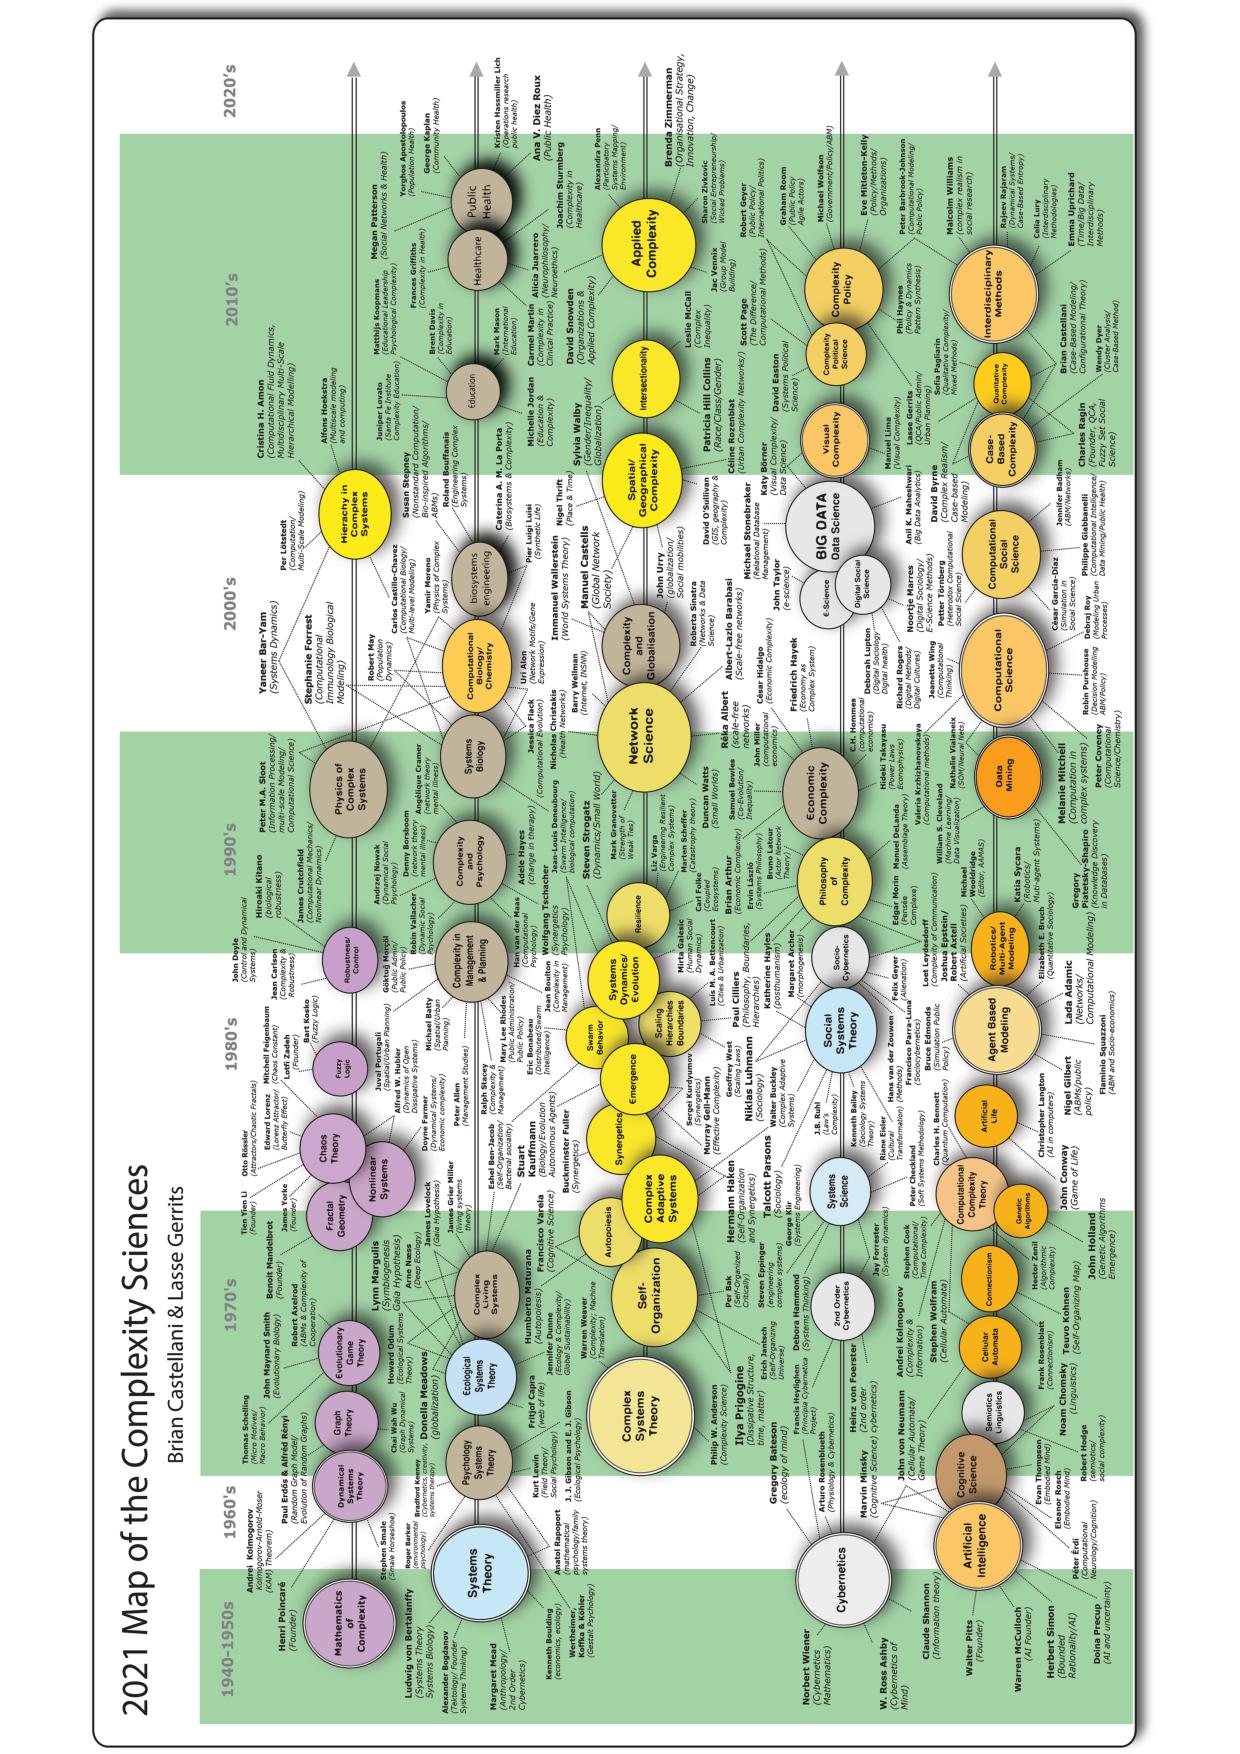
\includegraphics[width=1.0\textwidth, angle=0]{figures/complexitymap.pdf}
    \caption{B.Castellani e L.Gerrits Mappa delle Scienze Complesse}
    \label{fig:figure}
\end{figure}
%% https://www.art-sciencefactory.com/MapLegend.html

\clearpage

\subsection{Le cibernetiche nella musica}
\label{sec:Le cibernetiche nella musica}
All'inizio degli anni '60 in seno alle nascita delle scienze complesse,
l'uso di sistemi di feedback e la rilevanza dei circuiti informativi chiusi
nelle strutture organizzate,
ha goduto di uno slancio popolare anche nel mondo della musica e più in generale dell'arte.
Uno dei primi nella storia dell'arte ad evocare l'uso della cibernetica nei propri lavori è stato
Nicolas Schoeffer con il suo ciclo di lavori "spazio-dinamici", in particolare ha creato
la prima installazione ad implementare meccanismi di auto-regolazione, il CYSP-1,
capace di essere sensibile all'ambiente esterno e a se stesso
grazie ad una serie di tecnologie offerte dalla compagnia Philips (fotocellule e microfoni),
e reagire sonoramente a questi stimoli riproducendo
una serie di registrazioni composte dal compositore francese Pierre Henry,
collaboratore di Pierre Schaeffer ed insieme a lui figura centrale nella nascita della Musique concrète.
Un'altra importante esperienza del periodo iniziale è quella del compositore Roland Kayn,
che dopo essersi avvicinato alla musica elettronica sotto la guida di Herbert Eimert
nello studio di Colonia (1954),
e dopo essersi trasferito a Roma nel 1960, dal 1964 assieme ad Aldo Clementi e Franco Evangelisti
fonda il Gruppo di improvvisazione Nuova Consonanza, del quale fece parte sino al 1968,
ed in quel periodo ispirato dalle teorie della cibernetica iniziò a sperimentare
estensivamente con sistemi di autoregolazione basati su feedback loops,
sia come modelli formali per composizioni strumentali che come reti di generatori di segnale analogici.
Tuttavia, a parte casi popolari di deliberate dichiarazioni formali da parte degli artisti,
come è nel caso di Roland Kayn,
non bisogna pensare a questi lavori appena citati (ed altri riportati a seguito),
come ad atti pioneristici che sancisono la nascita della cibernetica in musica,
ma proprio come si dice per la scoperta del fuoco
lo scenario più accurato risiede probabilmente nel fatto che
tanti autori provenienti da diverse parti del mondo, nello stesso periodo
sono stati influenzati e si sono influenzati a vicenda con le stesse idee
provenienti da un interesse condiviso per le teorie cibernetiche di Weiner e delle Macy Conferences.
Si può pensare ad esempio a quelle che sono le esperienze dello studio di Colonia:
nel 1951, Herbert Eimert e Werner Meyer-Eppler persuasero il direttore della NWDR, Hanns Hartmann,
a creare uno Studio per la Musica Elettronica, che Eimert diresse fino al 1962.
Questo è diventato lo studio più influente al mondo durante gli anni 1950 e 1960,
con ospiti alcuni dei più importanti compositori contemporanei provenienti da tutta europa,
come il già citato Roland Kayn, Franco Evangelisti, Karlheinz Stockhausen, Herbert Brun,
Cornelius Cardew, e molti altri.
Qui è dove nel 1964 K.Stockhausen lavora a Mikrophonie I, che seppure non dichiarato è un ovvio punto di inizio
se si pensa a quelle logiche di interazione sistemiche fra uomo/macchina/ambiente in musica,
e in quel caso un punto di formalizzazione importante per quella che sarà l'esperienza del live electronics,
e non a caso in quel periodo il lavoro di ricerca condotto da Werner-Meyer Eppler,
scienziato, musicista ideatore e direttore dello studio di Colonia,
ha trovato sin dalla nascita dello studio fondamento in quelle che sono state
le teorizzazioni della Cibernetica.
Per continuare, parlando sempre dello studio di colonia, c'è il caso di Franco Evangelisti,
come citato prima fondatore insieme a Roland Kayn del Gruppo Improvvisazione Nuova Consonanza,
che in quel periodo (qualche anno prima della fondazione del gruppo a Roma)
si trova nello studio di Colonia per lavorare al brano: Incontri di Fasce Sonore,
e quando farà ritorno a Roma poi citerà più volte deliberatamente in interviste, scritti,
e altre documentazioni, il suo approccio sistemico/cibernetico a quelle che sono le esperienze con
Gruppo.
O ancora, se cambiamo rete e passiamo dall'Europa od osservare l'America in quel periodo,
possiamo pensare a quelli che sono i lavori di Louis e Bebe Barron,
con i circuiti in retroazione destinati al corto circuito
e utilizzati appositamente come materiale per la generazione acustica di trame incise su nastro,
o al lavoro di Alvin Lucier, che nel 1969 scriverà quello che sarà un brano emblematico per
la cibernetica in musica: I'm sitting in a room, altro brano importante per quelle che sono
le logiche di interazione sistemiche fra uomo/macchina/ambiente e che sancisce una volta per tutte
l'interazione sistemica dove il musicista, l'ambiente e lo strumento sono parti di un insieme del
sistema "più complesso" con un comportamento collettivo derivato dai singoli agenti.
Dunque la cibernetica da teoria scientifica diviene nel dopoguerra
l'elemento che tesse alcune delle più importanti trame all'interno dell'ambiente
nascente della musica elettronica.
